%------------------------------------------------------------------------------%
%                                     FDS                                      %
%------------------------------------------------------------------------------%

\section{FDS}
\label{sec:fds}

In this section, we will explain what \gls{fds} is, and we will describe some of
the work that has been done on this tool.

\subsection{The Fire Dynamics Simulator}
\label{sec:fdsdesc}

"\gls{fds} is a computational fluid dynamics (CFD) model of fire-driven fluid
flow. The FDS software solves numerically a form of the Navier-Stokes
nist-equations appropriate for low-speed, thermally-driven flow, with an
emphasis on smoke and heat transport from fires" \cite{fds:pres}. The first
version of the simulator was published in February 2000. It is used for solving
practical problems in fire protection engineering and to study fundamental
fire dynamics and combustion \cite{fds:tutorial}.

The simulator program reads the configuration from a text file that describes
the parameters, computes the solution of the equations and writes the results to
different files. The format of the configuration file is described in the user's
guide \cite{fdsguide}. The output files of the simulator can either be analyzed
directly or they can be used as input for other programs. Indeed, \gls{fds} can
be paired with two other programs. Evac is the evacuation simulation module for
\gls{fds}; it is used to simulate the movement of people in evacuation
situations \cite{fds:evac}. Smokeview is a visualization program that displays
the output of \gls{fds}. The figure \ref{fig:smvexample} shows an example of the
Smokeview's output. The usage of this tool is described in \cite{smvguide}.

% [Smokeview example] {{{
\begin{figure}[h!]
  \begin{center}
    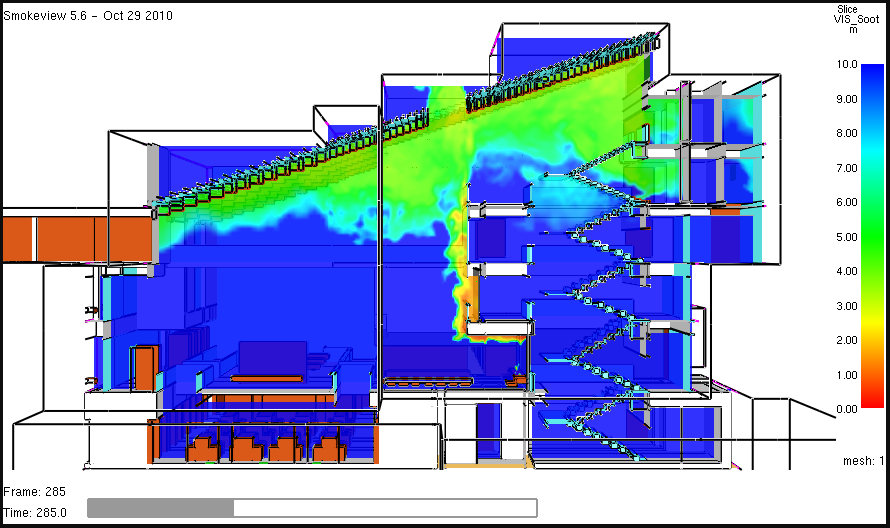
\includegraphics[scale=0.5]{img/smvexample.png}
    \caption{Smokeview example}
    \label{fig:smvexample}
  \end{center}
\end{figure}
%}}}

During the project, neither Evac nor Smokeview were used. However, it is
still useful to mention them to provide some context.

\gls{fds} uses a large-eddy simulation (LES) model \cite{fdsref}, which is a
mathematical model for turbulence used in computational fluid dynamics
\cite{enwiki:les}. This is an alternative to direct numerical simulation (DNS)
when the computational costs become too high. The idea is to ignore the small
elements by utilizing a low-pass filter on the equations to simplify the
computation \cite{enwiki:les} and \cite{ferziger1996large}. The small elements
can still have an effect on the solution. To solve this problem, \gls{fds}
simulation is divided in two parts as described in the technical reference
\cite{fdsref}. First the predictor part estimates the terms at the next time
step. At the end of the predictor, the simulator verifies the stability
conditions. If the stability conditions are satisfied, the predictor proceeds to
the next time step. Otherwise, the corrector adjusts the terms before the
simulation continues to the next time step. Both of these steps will be
represented as sub-graphs in the \gls{hh} version of the simulator. The
\gls{fds}'s simulation has many other characteristics that will not be detailed
in this report. However, all the mathematical tools and models used by the
simulators are detailed by \cite{fdsref}.

The simulation is written entirely in Fortran (standard 2018). The code is
already parallelized using MPI and OpenMP. MPI is used to parallelize the
computation of the meshes \footnote{As explained in the user's guide, a mesh is a
portion of the 3D space. Normally, they are used for modeling complex geometrical
structures that do not fit in one parallelogram (corridors for instance).
However, they can also be used to perform a block decomposition on the
matrices.} on multiple nodes on a cluster, and OpenMP is used to parallelize
many of the loops that are present in the program. Interestingly, \gls{fds} does
not use any other dependencies such as \textit{BLAS} or \textit{LAPACK} that
we used in the Cholesky implementation. Furthermore, the simulator is not yet
capable of performing GPU computation. However, the developers are interested in
using GPUs in the \gls{hh} implementation.

Now that we have described what \gls{fds} is, let us see what has been done to
optimize the simulation with \gls{hh}.

\subsection{3D loops}

One of the bottlenecks of the simulation is the computation of the velocity.
This part of the program consists of three 3D loops that iterates on the tensors
of each mesh, and can be used several times during a tick of the simulation.
Since it is a critical part of the program, the developers of \gls{fds} have
created a test program, separated from the full simulation, that is used to
measure and try various optimizations. This test program has been very useful in
the effort of optimizing the simulation with \gls{hh} since it was simpler
compared to the simulator itself. In this section, we will describe the test
program developed by the \gls{fds}'s developers. Then we will explain how the
computation of the velocity has been optimized using block decomposition.
Finally, we will discuss the limitations of the method that has been used.

\subsubsection{The test program}

As mentioned in the introduction of the section, the test program includes
only the part of the simulation responsible for the computation of the velocity.
The program consists in three 3D loops parallelized with OpenMP. These loops
are independent, so they are in a parallel section and there are no barriers
between the loops (they run in parallel). Listing \ref{lst:3Dloopscode}
shows the loops with the OpenMP pragmas (note that all the nested loops are not
represented here).

%- begin listing ------------------------------------------------------------{{{
\begin{listing}[ht!]
\begin{minted}[frame=lines,framesep=2mm,baselinestretch=1.2,fontsize=\normalsize,linenos]{Fortran}
! Compute x-direction flux term FVX

!$OMP PARALLEL PRIVATE(...)
!$OMP DO SCHEDULE(STATIC) PRIVATE(WOMY, VOMZ, TXXP, TXXM, DTXXDX, DTXYDY, DTXZDZ)
DO K=1,KBAR
   ! ...
ENDDO
!$OMP END DO NOWAIT

! Compute y-direction flux term FVY
!$OMP DO SCHEDULE(STATIC) PRIVATE(WOMX, UOMZ, TYYP, TYYM, DTXYDX, DTYYDY, DTYZDZ)
DO K=1,KBAR
   ! ...
ENDDO
!$OMP END DO NOWAIT

! Compute z-direction flux term FVZ
!$OMP DO SCHEDULE(STATIC) PRIVATE(UOMY, VOMX, TZZP, TZZM, DTXZDX, DTYZDY, DTZZDZ)
DO K=0,KBAR
   ! ...
ENDDO
!$OMP END DO NOWAIT
!$OMP END PARALLEL
\end{minted}
\caption{3D loops source code}
\label{lst:3Dloopscode}
\end{listing}
%- end listing --------------------------------------------------------------}}}

The test program is divided in two parts. In the first part, all the variables
are initialized. We will not explain the initialization since it is not present
in the simulator. This initialization is just used to have values on which we
can perform computation. The second part of the program is the computation of
the velocity. We measure the computation time for this section. Finally, the
program calculates the mean for each direction (\texttt{FVX}, \texttt{FVY} and
\texttt{FVZ}) in order to have simple values that can be easily verified. The
computation time of the mean is not taken into account when we make the measure
on the original test program, unlike in the \gls{hh} one. We will explain why
the \gls{hh} program measures the computation of the mean as well in the section
\ref{sec:3Dloopsmethod}. Finally, like in the \gls{fds}'s code, most of the
variables are global, which makes difficult to analyze the dependencies between
the tasks.

\subsubsection{The method}
\label{sec:3Dloopsmethod}

To introduce \gls{hh} in this first part of the simulation, the goal was to keep
the entire computation in Fortran. The objective was to be efficient and avoid
rewriting the code in C++. Furthermore, all the variables have been kept in
Fortran as well. Here, \gls{hh} serves as an orchestrator, responsible for
allocating and managing the threads in which the Fortran subroutines are called
when it is required. All the OpenMP pragmas have been removed since we do not
want to perform fine grain parallelism, we want the threads to be entirely
managed by \gls{hh}.

As mentioned in the introduction of this section, to optimize computation time,
we have used block decomposition on the 3D arrays of the simulation. In order to
do this, the Fortran code was reorganized in subroutines that are parametrized
with the boundaries. The declarations of these new subroutines are shown in the
listing \ref{lst:looproutines}. Here we can see as well that we use the ISO C
bindings to be able to call the subroutines from C++. The original loops have
been moved in the new subroutines, and modified to iterate over the blocks
instead of the whole matrix. \clearpage{}

%- begin listing ------------------------------------------------------------{{{
\begin{listing}[ht!]
\begin{minted}[frame=lines,framesep=2mm,baselinestretch=1.2,fontsize=\normalsize,linenos,breaklines=true]{Fortran}
SUBROUTINE COMPUTE_X_FLUX(IBEGIN, JBEGIN, KBEGIN, IEND, JEND, KEND) BIND(C, NAME = "computeXFlux")
SUBROUTINE COMPUTE_Y_FLUX(IBEGIN, JBEGIN, KBEGIN, IEND, JEND, KEND) BIND(C, NAME = "computeYFlux")
SUBROUTINE COMPUTE_Z_FLUX(IBEGIN, JBEGIN, KBEGIN, IEND, JEND, KEND) BIND(C, NAME = "computeZFlux")
\end{minted}
\caption{Loop subroutines signature}
\label{lst:looproutines}
\end{listing}
%- end listing --------------------------------------------------------------}}}

Listing \ref{lst:loophhtask} illustrates how the subroutines are used in the
\gls{hh} tasks. Here, we can see that the tasks take a block index as input. As
explained earlier, the graph only manages blocks indices. Each block has the
start index and the end index on each dimension. In order to send the right
blocks to the right tasks, the block type includes an identifier as template
parameter. This identifier indicates whether the block should be used to
compute the $x$, $y$ or $z$ direction. In the case shown bellow, we want to
compute the terms on the $x$ axis, so the identifier of the block is \texttt{X}.
The same block is transmitted to the \texttt{Y} and \texttt{Z} tasks
using the corresponding identifiers.

%- begin listing ------------------------------------------------------------{{{
\begin{listing}[ht!]
\begin{minted}[frame=lines,framesep=2mm,baselinestretch=1.2,fontsize=\normalsize,linenos]{C++}
  void execute(std::shared_ptr<BlockIdx<X>> block) override {
    size_t i = block->i == 1 ? 0 : block->i;
    computeXFlux(&i, &block->j, &block->k,
                 &block->iEnd,
                 &block->jEnd,
                 &block->kEnd);
    this->addResult(block);
  }
\end{minted}
\caption{Hedgehog compute task for the 3D Loops program.}
\label{lst:loophhtask}
\end{listing}
%- end listing --------------------------------------------------------------}}}

The figure \ref{fig:loopsgraph} shows that the \gls{hh} graph has three steps:

\begin{itemize}
  \item Initialization: creation of the block indices (has previously
    mentioned, \gls{hh} manages only indices and not the actual data).
  \item Computation of the velocity: this part holds the loops that compute the
    velocity for the x, y and z axis. There is one task per axis, and these
    tasks call the Fortran subroutines with the blocks boundaries. As shown in
    the graph, all those three tasks are executed in parallel.
  \item Computation of the mean
\end{itemize}
\clearpage{}

% [3D loops graph] {{{
\begin{figure}[h!]
  \begin{center}
    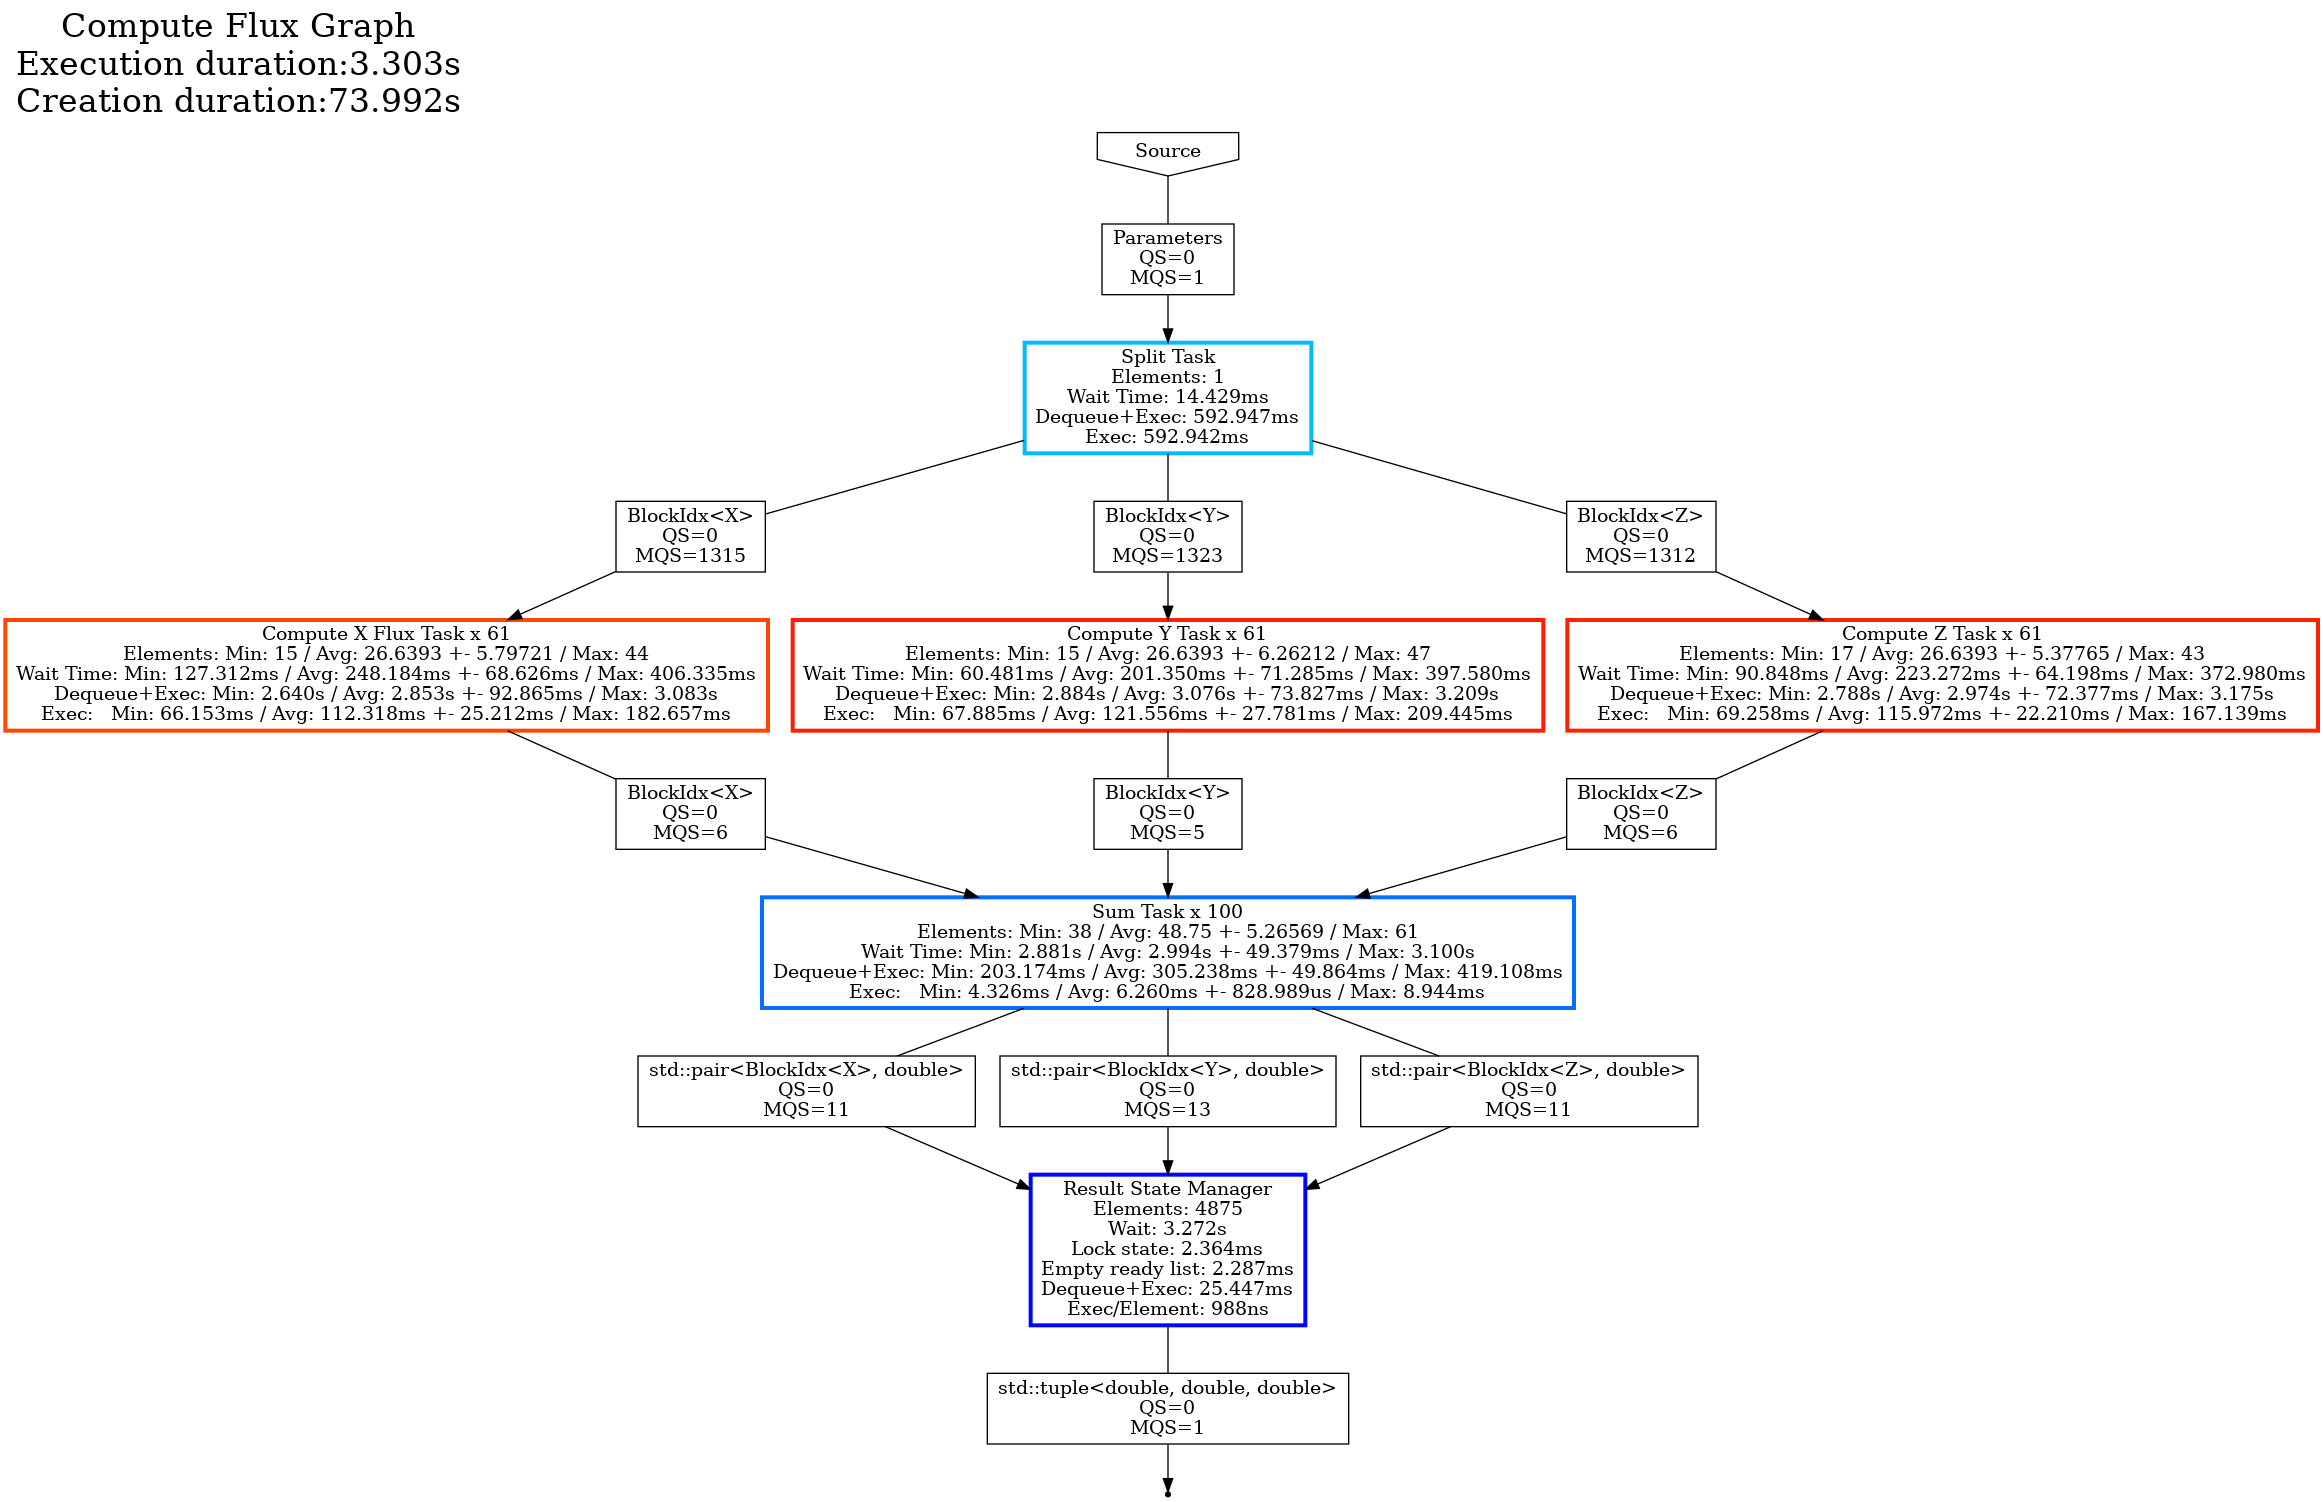
\includegraphics[scale=0.2]{img/fds-loops/graph-61.png}
    \caption{3D loops graph}
    \label{fig:loopsgraph}
  \end{center}
\end{figure}
%}}}

It would have been possible to use a single task to perform all the computations
for the three axis. However, using three separated tasks means that we also have
three queues of data. If only one tasks was used, all the blocks for each axis
would be in the same queue. To optimize the dequeue times, we use multiple tasks
running in parallel, with each task having its own queue.

\subsubsection{The results}

Now that we have explained how the graph has been implemented, we can describe
the results. Before we start, it is important to mention that the measurements
were taken on a node that has 384 threads, however, here, only 200 threads where
available. Another important detail concern the problem size. In order to test
the limits of the algorithm, the measures have been made on very big matrices
($1024\times1024\times1024$). This size is much larger compared to the size of
the meshes that the algorithm will treat in reality. Making the measures on such
a problem allows having more distinguishable differences between the programs,
and helps to see if the program scales effectively.

Firstly, the plot \ref{fig:loopscomptime} shows the computation of the two
programs. As we can see, the \gls{hh} program is faster than the \gls{fds} one.
Furthermore, as shown by the standard deviation, it is also much more
consistent. This demonstrates that using block decomposition improves the speed
and the consistency of the program. \clearpage{}

% [Computation times] {{{
\begin{figure}[ht!]
  \begin{center}
    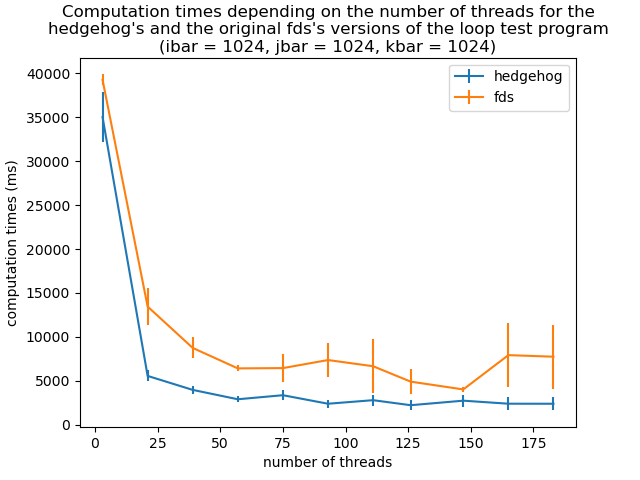
\includegraphics[scale=0.6]{img/fds-loops/times.png}
    \caption{Computation times of the test program for HH and FDS (200 threads node)}
    \label{fig:loopscomptime}
  \end{center}
\end{figure}
%}}}

Figure \ref{fig:loopsspeedup} shows the acceleration of the
\gls{hh} program compared to the \gls{fds} one. We can notice that on the point
were \gls{fds} shows its best performance, \gls{hh} is nearly two times faster.
Interestingly, \gls{fds} starts to be very unstable with more than 150 threads,
which results in a very high speedup of the \gls{hh} program.

% [Acceleration] {{{
\begin{figure}[ht!]
  \begin{center}
    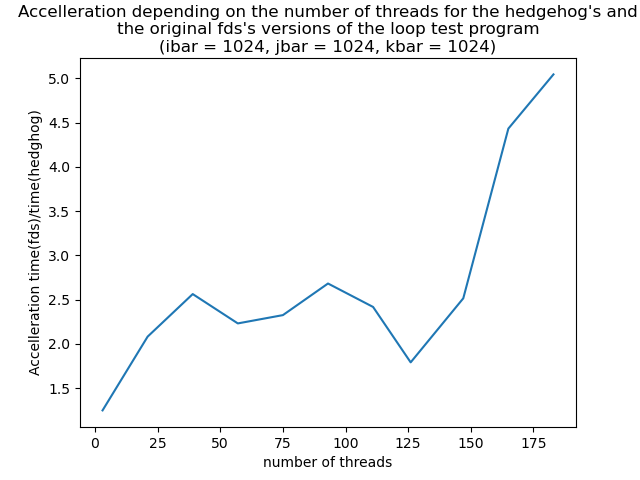
\includegraphics[scale=0.6]{img/fds-loops/speedup.png}
    \caption{Acceleration of HH over FDS on the test program (200 threads node)}
    \label{fig:loopsspeedup}
  \end{center}
\end{figure}
%}}}

Finally, Figure \ref{fig:loopsrelativespeedup} shows the relative speedup for
each program. This relative speedup is not very high for both of the programs,
indicating that we have not achieved sufficient parallelism \footnote{In this
context, achieving high degree of parallelism means utilizing all the resources
of the processors.} yet. For \gls{hh} this can be explained by the fact that the
chosen block size is not optimal. In these measurements, the block size was
($1024\times32\times1$), which might be either too large or too small.
Generally, finding the optimal block size is difficult as there are no
definitive methods to determine it. The usual approach is to test the program
with various block sizes. However, this was difficult to do on this program
considering the fact that the initialization is very slow. It took more than
twenty hours of computation to obtain the measurements presented in this
section.

% [Relative speedup] {{{
\begin{figure}[ht!]
  \begin{center}
    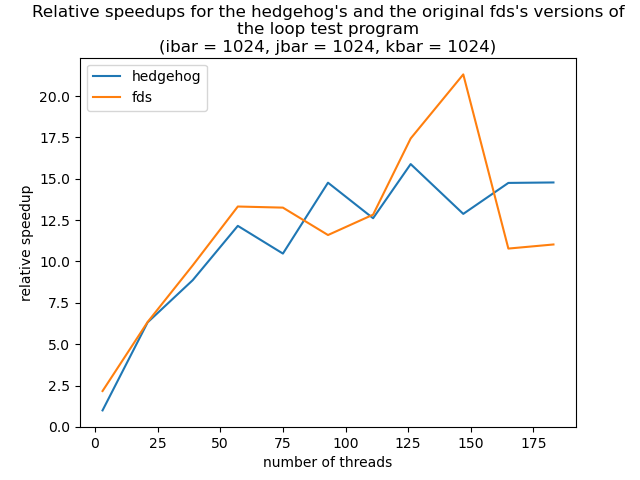
\includegraphics[scale=0.6]{img/fds-loops/relative_speedup.png}
    \caption{Relative speedup for HH and FDS on the test program (200 threads node)}
    \label{fig:loopsrelativespeedup}
  \end{center}
\end{figure}
%}}}

Ultimately, these results demonstrate that the block decomposition can have a
significant impact on the computation time. Furthermore, testing this program
permitted to understand how to use Fortran and C++ together. In the next
section, we will explain why this method cannot be applied to the global
simulation.

\subsubsection{Limitations}

This method is effective and relatively easy to set up, however it still has
some limitations.

Firstly, the fact that the data is entirely managed by Fortran poses a problem.
Indeed, \gls{hh} creates a data-flow graph, so it should be responsible for
managing all the data. This would not have a significant impact on the
performance, but it would improve the readability of the graph, as it would
allow to clearly see which task access which data. Having a clear and well
organized graph is very important to keep the application maintainable and
expandable.

Secondly, with this method, it is not easy to have computation in C++. As
discussed the section \ref{sec:cholesky}, some parts of the code were completely
rewritten in C++. Keeping all the data as global variables in Fortran
complicated the usage of pure C++ or external \footnote{Here, external means
that the sub-graphs uses other languages.} sub-graphs. The data that flows into
the global graph should not be defined in both languages, otherwise, this would
require to have synchronisation tasks for copying the data between them. Such
tasks would have a significant impact on the performance.

Finally, it may not always be possible to keep the types as they currently are
in \gls{fds}. Indeed, explained in the section \ref{sec:fdsdesc}, the simulator
performs computation on meshes and this computation can be done on multiple
node. Since these meshes belong to the same geometrical area, after each
computation, we need to synchronise the modifications make to the
stencils \footnote{Area around a mesh that is shared with other meshes} of the
meshes. This problem will also be present with the blocks on the \gls{hh}
version. To perform the update efficiently, we will need to have a data
structure that will represent the stencils, which does not
exist in the \gls{fds} code yet. Moreover, it is preferable not to implement
this data structure in Fortran. Firstly because it might be more difficult to
implement (Fortran does not have all the tools that C++ has), and secondly
because the code that will perform the update will be easier to write in C++.

Working on this example program was very useful, primarily as it helped to
understand some parts of the code. Furthermore, this was a good demonstration
of what could be done with \gls{hh} on the \gls{fds} code, and it allowed us to
experiment with a part of the code extracted from the whole simulation.
Unfortunately, the method that has been used here cannot be utilized for
parallelizing the rest of the program, but we learned a lot from this exercise.

\subsection{Conclusion}
\label{sec:fdsconcl}

So far, we have seen the work that has been done on different parts of the
simulation. These parts have been treated separately to try different methods
for optimizing the entire code. We have demonstrated that it is possible to
rewrite some sections entirely in C++, such as the Cholesky decomposition. We
also experimented using \gls{hh} as an orchestrator while keeping all the
computation and the memory in Fortran, and we have seen why this is eventually
the ideal approach.

To parallelize the entire simulation with \gls{hh} we have tried to tackle the
problem from two sides. First, we aimed to parallelize specific pieces of the
application, as we did for the velocity. Second, we focus on creating a global
graph and try to set up a pipeline threw the entire simulation. The role of the
global graph is to call Fortran subroutines. The gaol is to refactor the graph
in order to have more specific tasks after each iteration. For instance, we
start by having a graph that calls a main function in Fortran. Then we refactor
this graph into a new one that has three tasks: the initialization, the main
loop and the end of the program. Then we try to split each of these three tasks
into sub-tasks to create a new graph, and we keep iterating till our tasks are
precise enough. Eventually, we should end up having atomic tasks, and some of
them can be run in parallel.

This approach was logical, however, implementing everything manually is
difficult due to the complexity and the size of the code base (more than 160K
lines of code). Furthermore, doing this manually is not a method that is easily
reproducible. For this reason, we have decided to try building a tool able to
perform some automatic transformations on the code. The specifications of the
tool will be described in the next section.
